% !TEX program = lualatex
%==============================================================================
%  The Global Matrix Method and the Source Jump.
%  The stratified reference solver: block-tridiagonal global matrix, the
%  Riccati reduction, and delta(z - z_1) I_6 as the source primitive.
%
%  Self-contained LuaLaTeX source. Compile with:
%      latexmk -lualatex GlobalMatrixMethod.tex
%==============================================================================
\documentclass[11pt,a4paper]{article}

% --- LuaLaTeX font handling -------------------------------------------------
\usepackage{fontspec}
\setmainfont{Latin Modern Roman}

% --- Mathematics ------------------------------------------------------------
\usepackage{amsmath}
\usepackage{amssymb}
\usepackage{mathtools}

% --- Layout and typography --------------------------------------------------
\usepackage[margin=1in]{geometry}
\usepackage{microtype}
\usepackage{xcolor}
\usepackage{booktabs}

% --- Graphics ---------------------------------------------------------------
\usepackage{tikz}
\usetikzlibrary{arrows.meta,positioning,fit,backgrounds}

% --- Hyperlinks -------------------------------------------------------------
\usepackage[colorlinks=true,
            linkcolor=blue!55!black,
            citecolor=blue!55!black,
            urlcolor=blue!55!black]{hyperref}
\hypersetup{
  pdftitle={The Global Matrix Method and the Source Jump},
  pdfauthor={Tod Nestor}
}

% --- Macros -----------------------------------------------------------------
\newcommand{\ii}{\mathrm{i}}
\newcommand{\rd}{\mathrm{d}}
\newcommand{\bI}{\mathbf{I}}
\newcommand{\bJ}{\mathbf{J}}
\newcommand{\bD}{\mathbf{D}}
\newcommand{\bE}{\mathbf{E}}
\newcommand{\bG}{\mathbf{G}}
\newcommand{\bY}{\mathbf{Y}}
\newcommand{\bb}{\mathbf{b}}
\newcommand{\bv}{\mathbf{v}}
\newcommand{\bS}{\boldsymbol{\Sigma}}
\newcommand{\kpar}{\mathbf{k}_{\parallel}}

\title{\bfseries The Global Matrix Method and the Source Jump\\[4pt]
\large The stratified reference solver, and
$\delta(z-z_1)\,\bI_6$ as its source primitive}
\author{Tod Nestor}
\date{14 September 2026}

\begin{document}
\maketitle

\begin{abstract}
The stratified reference medium of the multiple-scattering programme is solved
by a global matrix: one block-tridiagonal system per horizontal wavenumber and
frequency, assembled from layer eigenvectors and interface continuity, and
reduced to an $O(N)$ sweep by a block-Riccati recursion. This note states that
construction as implemented, and then addresses the part of it that has never
been written down completely --- the source. A source enters the global matrix
as a \emph{jump} in the six-component state across its own plane. We show that
the up- and down-going radiation produced by the unit jump
$\delta(z-z_1)\bI_6$ is exactly the inverse eigenvector matrix, available in
closed form without a linear solve, because the layer modes are symplectically
orthogonal. One matrix therefore yields every column of the Green's function at
once. The existing treatment restricts the source to the free-surface layer or
the lower half-space; the unit jump removes that restriction.
\end{abstract}

\bigskip
\noindent\textbf{Companion series.}\enspace{\small\itshape One of a companion
series on elastic multiple scattering from cubic heterogeneities on a
depth-stratified background, the T-matrix programme
$T=T_0(I-G_0T_0)^{-1}$. This note covers the \emph{reference} solver: the
stratified medium on which the scattering series is built. Its companions treat
the inter-site propagator, the contrast-source volume integral equation, and the
directional partial-wave sweep matvec.}

\tableofcontents
\bigskip

%==============================================================================
\section{The stratified system}
%==============================================================================

Work at fixed angular frequency $\omega$ and fixed horizontal wavenumber
$\kpar=(k_x,k_y)$, with the time convention $e^{-\ii\omega t}$, depth $z$
positive downward, and seismic units (km\,s$^{-1}$, g\,cm$^{-3}$, GPa, km). The
medium is a stack of homogeneous layers; within each, the displacement and
traction satisfy a first-order system in $z$ whose solutions are plane waves.

The natural dependent variable is the six-component \emph{state}
\begin{equation}\label{eq:state}
  \bv(z) \;=\; \bigl(u_z,\;u_x,\;u_y,\;\tau_{zz},\;\tau_{xz},\;\tau_{yz}\bigr)^{\mathsf T},
\end{equation}
because exactly these six quantities are continuous across a welded interface.
Everything else --- the in-plane strains, the remaining stress components ---
jumps with the material, and any formulation carrying them across an interface
has to undo that jump again.

In each layer the system supports six modes: $P$, $SV$ and $SH$, each up- or
down-going. Collecting their state vectors as the columns of a matrix
$\bD_z(\kpar)$, the field in layer $j$, spanning $z_j\le z\le z_{j+1}$, is
\begin{equation}\label{eq:layerfield}
  \bv(z) \;=\; \bD_{z}^{(j)}\,
  \begin{pmatrix}\mathrm{e}^{+\ii\omega\eta\,(z-z_j)}\,\mathbf{c}_{\downarrow}\\[2pt]
                 \mathrm{e}^{-\ii\omega\eta\,(z-z_{j+1})}\,\mathbf{c}_{\uparrow}\end{pmatrix},
\end{equation}
with $\eta$ the vertical slowness of the mode in question, on the branch
$\operatorname{Im}\eta\ge0$.

\paragraph{Each amplitude is referenced to the boundary its wave starts from.}
This is not cosmetic, and it is the single most important convention in the
whole construction. The down-going amplitude $\mathbf{c}_{\downarrow}$ is
referenced at the \emph{top} $z_j$ and the up-going amplitude
$\mathbf{c}_{\uparrow}$ at the \emph{bottom} $z_{j+1}$, so that both exponents
in \eqref{eq:layerfield} have the form $+\ii\omega\eta\times(\text{positive
distance travelled})$. Writing $\eta=\eta_r+\ii\eta_i$ with $\eta_i\ge0$, each
factor is then
\[
  \mathrm{e}^{\ii\omega\eta_r d}\,\mathrm{e}^{-\omega\eta_i d},\qquad d>0,
\]
which \emph{decays}. Referencing the up-going wave to the top instead --- the
apparently symmetric choice $\mathrm{e}^{-\ii\omega\eta(z-z_j)}$ --- gives
$\mathrm{e}^{+\omega\eta_i d}$ and builds a growing exponential into the
formulation. For propagating wavenumbers the difference is a bookkeeping
convention; for evanescent ones, where $\eta_i$ is large and $\omega\eta_i h$
may be tens or hundreds, it is the difference between a stable recursion and an
overflow. The growing exponential is never formed anywhere in this construction,
and \eqref{eq:layerfield} is where that begins.

The amplitudes $\mathbf{c}_{\downarrow},\mathbf{c}_{\uparrow}$ are the unknowns.
Every phase factor that appears below is consequently
$\mathrm{e}^{+\ii\omega\eta h}$ with $h>0$ a layer thickness or a fraction of
one: a single layer crossing, always in the decaying direction.

\paragraph{Decoupling.} At fixed $\kpar$ the six modes separate into a
four-component $P$--$SV$ system in the sagittal plane and a two-component $SH$
system out of it, related to the Cartesian state by a rotation through the
azimuth $\phi=\arctan(k_y/k_x)$. The implementation carries the two blocks
separately and rotates on output. The $P$--$SV$ state is
$(u_x,u_z,\tau_{zz}/(-\ii\omega),\tau_{xz}/(-\ii\omega))$ and the $SH$ state is
$(u_t,\tau_{tz}/(-\ii\omega))$; the $(-\ii\omega)$ scaling keeps the layer
matrices frequency-independent.

%==============================================================================
\section{The global matrix}
%==============================================================================

Continuity of $\bv$ at every interface, together with the free surface above and
the radiation condition below, closes the system. Writing the layer amplitudes
as the unknown vector and continuity as the equations, the result is one linear
system per $(\omega,\kpar)$,
\begin{equation}\label{eq:global}
  \mathcal{A}\,\mathbf{c} \;=\; \bb,
\end{equation}
whose matrix is \emph{block tridiagonal}: interface $k$ couples only the
amplitudes of the layers immediately above and below it.

\begin{figure}[h]
\centering
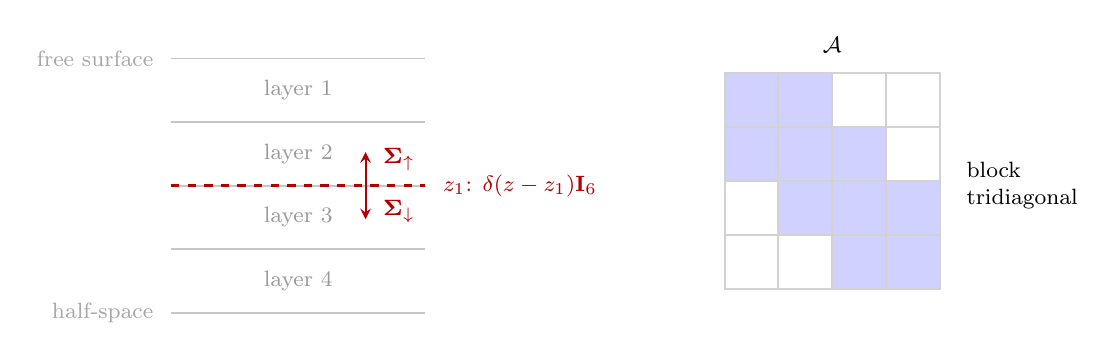
\begin{tikzpicture}[>=stealth, line width=0.7pt, scale=0.95]
  % layer stack on the left
  \foreach \i/\lab in {0/{free surface}, 1/{}, 2/{}, 3/{}, 4/{half-space}}{
    \draw[gray!45] (0,-\i*0.85) -- (3.4,-\i*0.85);
  }
  \node[gray!70, anchor=east, font=\footnotesize] at (-0.1, 0) {free surface};
  \node[gray!70, anchor=east, font=\footnotesize] at (-0.1,-3.4) {half-space};
  \foreach \i/\lab in {0/1, 1/2, 2/3, 3/4}{
    \node[font=\footnotesize, gray!80] at (1.7,-\i*0.85-0.42) {layer \lab};
  }
  % source plane
  \draw[red!70!black, dashed, line width=1pt] (0,-1.7) -- (3.4,-1.7);
  \node[red!70!black, anchor=west, font=\footnotesize] at (3.5,-1.7)
       {$z_1$: $\delta(z-z_1)\bI_6$};
  \draw[->, red!70!black] (2.6,-1.7) -- (2.6,-2.15);
  \draw[->, red!70!black] (2.6,-1.7) -- (2.6,-1.25);
  \node[red!70!black, font=\footnotesize, anchor=west] at (2.7,-2.05) {$\bS_{\downarrow}$};
  \node[red!70!black, font=\footnotesize, anchor=west] at (2.7,-1.35) {$\bS_{\uparrow}$};

  % block tridiagonal matrix on the right
  \begin{scope}[xshift=7.4cm, yshift=-0.2cm]
    \foreach \i in {0,...,3}{
      \foreach \j in {0,...,3}{
        \pgfmathparse{abs(\i-\j)<=1 ? 1 : 0}
        \ifnum\pgfmathresult=1
          \fill[blue!18] (\j*0.72,-\i*0.72) rectangle ++(0.72,-0.72);
        \fi
        \draw[gray!35] (\j*0.72,-\i*0.72) rectangle ++(0.72,-0.72);
      }
    }
    \node[font=\footnotesize, anchor=south] at (1.44,0.15) {$\mathcal{A}$};
    \node[font=\footnotesize, anchor=west] at (3.1,-1.5)
         {\begin{tabular}{@{}l@{}}block\\tridiagonal\end{tabular}};
  \end{scope}
\end{tikzpicture}
\caption{Left: the layer stack, with a source plane at $z_1$ radiating
$\bS_{\uparrow}$ upward and $\bS_{\downarrow}$ downward. Right: the global
matrix $\mathcal{A}$ of \eqref{eq:global}. Each interface couples only
neighbouring layers, so $\mathcal{A}$ is block tridiagonal --- which is what the
Riccati recursion of \S\ref{sec:riccati} exploits.}
\end{figure}

Solving \eqref{eq:global} densely costs $O(N^3)$ in the number of layers, and it
must be solved afresh for every frequency and every wavenumber. That cost is the
reason for the next section.

%==============================================================================
\section{The Riccati reduction}
\label{sec:riccati}
%==============================================================================

Block tridiagonality permits the standard elimination: sweep from the
half-space upward, carrying at each interface a single $2\times2$ matrix
$\bY_k$ that summarises everything below it. At interface $k$, with $\bE_d$ and
$\bE_u$ the down- and up-going eigenvector blocks and $\bE$ the layer phase,
\begin{equation}\label{eq:riccati}
  \bigl[\,\bE_u^{(k)} \;\; -\bE_{\text{eff}}^{(k+1)}\,\bigr]
  \begin{pmatrix}\bY_k\\ \ast\end{pmatrix}
  \;=\;-\,\bE_d^{(k)}\bE^{(k)},
  \qquad
  \bE_{\text{eff}}^{(k+1)} = \bE_d^{(k+1)} + \bE_u^{(k+1)}\bE^{(k+1)}\bY_{k+1},
\end{equation}
so each step is a $4\times4$ solve and the whole sweep is $O(N)$. $\bY_k$ is the
reflection matrix of the stack below interface $k$, and the recursion is the
matrix Riccati equation of invariant embedding.

Its stability is inherited directly from \eqref{eq:layerfield} rather than
imposed. Because $\mathbf{c}_{\downarrow}$ is referenced at the top of its layer
and $\mathbf{c}_{\uparrow}$ at the bottom, the phase $\bE^{(k)}$ multiplying
$\bE_d^{(k)}$ in \eqref{eq:riccati} carries the down-going wave from the top to
the bottom, and the phase multiplying $\bE_u^{(k+1)}$ carries the up-going wave
from the bottom to the top. Both are $\mathrm{e}^{+\ii\omega\eta h}$ with
$h>0$; both decay. No step of the sweep ever forms a growing exponential, which
is what lets it run to arbitrary evanescence without conditioning collapse.

A particular solution rides alongside the homogeneous sweep. Writing
$\mathbf{g}_k$ for the accumulated source contribution below interface $k$, the
same factorisation that gives $\bY_k$ gives $\mathbf{g}_k$ at no extra cost:
the right-hand side gains a column, and the $4\times4$ solve is performed once
against both. Sources therefore cost one extra column, not one extra sweep.

%==============================================================================
\section{The source as a jump}
\label{sec:jump}
%==============================================================================

Now the part that motivates this note.

A source does not enter \eqref{eq:global} as a right-hand side in the obvious
place. It enters as a \emph{discontinuity} in the state across its own plane: on
either side of $z_1$ the field is source-free and satisfies
\eqref{eq:layerfield}, and the source is the mismatch between the two
solutions,
\begin{equation}\label{eq:jumpdef}
  \bv(z_1^{+}) - \bv(z_1^{-}) \;=\; \mathbf{S}.
\end{equation}
Everything about a source is in that six-vector. A body force, a moment tensor,
an explosion and a stress glut differ only in the $\mathbf{S}$ they produce.

\paragraph{The unit jump.} It is therefore natural to take as the primitive not
any particular physical source but the \emph{unit} jump
\begin{equation}\label{eq:unitjump}
  \mathbf{S} \;=\; \delta(z-z_1)\,\bI_6 ,
\end{equation}
whose six columns are the six independent state discontinuities. The response to
\eqref{eq:unitjump} is the Green's function of the stratified medium: all six
source components at once, one object rather than six solves. Any physical
source is then a linear combination, formed \emph{after} the expensive part is
done.

\subsection{Decomposing the jump: symplectic orthogonality}

To use \eqref{eq:unitjump} the jump must be split into the amplitudes it
excites. With $\bE=[\,\bE_d\mid\bE_u\,]$ the full eigenvector matrix of the
source layer, the amplitudes $\mathbf{c}$ solve $\bE\,\mathbf{c}=\mathbf{S}$,
so for the unit jump
\begin{equation}\label{eq:cinv}
  \mathbf{c} \;=\; \bE^{-1}.
\end{equation}
That looks like a matrix inversion per frequency and per wavenumber. It is not,
and the reason is structural.

Define the symplectic form on the state,
\begin{equation}\label{eq:form}
  \langle \bb_1,\bb_2\rangle \;=\; \bb_1^{\mathsf T}\bJ\,\bb_2 ,
  \qquad
  \bJ=\begin{pmatrix}\mathbf{0}&\bI_3\\-\bI_3&\mathbf{0}\end{pmatrix},
\end{equation}
pairing each displacement component with its conjugate traction. The elastic
layer operator is Hamiltonian with respect to \eqref{eq:form}, and its
eigenvectors are consequently \emph{symplectically orthogonal}: the Gram matrix
\begin{equation}\label{eq:gram}
  \mathbf{G} \;=\; \bE^{\mathsf T}\bJ\,\bE
\end{equation}
is block-antidiagonal with \emph{diagonal} blocks. Each mode pairs with its own
opposite-going partner and with nothing else --- $P_{\downarrow}$ with
$P_{\uparrow}$, $S_{\downarrow}$ with $S_{\uparrow}$, never $P$ with $S$. From
\eqref{eq:gram} the inverse follows immediately:
\begin{equation}\label{eq:syminv}
  \boxed{\;\bE^{-1} \;=\; \mathbf{G}^{-1}\,\bE^{\mathsf T}\bJ\;}
\end{equation}
and $\mathbf{G}^{-1}$ is a block swap together with one reciprocal per mode. The
inversion has disappeared.

\paragraph{The same statement, in the energy-normalised basis.} When the
eigenvectors are scaled so that the pairings in \eqref{eq:gram} are unity, the
Gram matrix becomes $\bJ$ itself and \eqref{eq:syminv} reduces to
\begin{equation}\label{eq:d1def}
  \bD_z^{-1}(\kpar) \;=\; -\ii\,\bJ\,\bD_z^{\mathsf T}(-\kpar)\,\bJ ,
\end{equation}
the symplectic inverse. Equation \eqref{eq:syminv} is that identity written for
eigenvectors in whatever normalisation they happen to carry: the structure
survives any diagonal rescaling, so no special normalisation is required to use
it.

\subsection{What this replaces}

The existing treatment computes the up- and down-going radiation from a dipolar
body force $\mathbf{F}=\mathbf{F}_1\delta(z-z_S)+\mathbf{F}_2\delta'(z-z_S)$ as
\begin{equation}\label{eq:boxsource}
  \begin{pmatrix}\bS_{\uparrow}\\ \bS_{\downarrow}\end{pmatrix}
  \;=\;-\ii\,\bigl\langle\,\bD_{z,S}(-\kpar),\;
  \mathbf{F}_1+\mathbf{A}_S\mathbf{F}_2\,\bigr\rangle ,
\end{equation}
and then restricts attention to a source in the free-surface layer or the lower
half-space, for which the assembled right-hand side $\bb$ has a closed form.

Equations \eqref{eq:unitjump}--\eqref{eq:syminv} are \eqref{eq:boxsource} with
$\mathbf{F}_1=\bI_6$ and $\mathbf{F}_2=\mathbf{0}$, and they carry two
consequences. The source may sit at \emph{any} depth, interior layers included,
because nothing in the derivation referred to the boundaries. And the
combination $\mathbf{F}_1+\mathbf{A}_S\mathbf{F}_2$ need not be formed at all
when what is wanted is the Green's function itself: the unit jump is the
identity, and a particular physical source is applied afterwards as a linear
combination of columns.

\subsection{Placing the radiation}

With $\mathbf{c}=\bE^{-1}$ in hand, the down-going half is propagated to the
bottom of the source layer and the up-going half to the top, each by its own
phase factor, and the two enter the Riccati right-hand side at the interfaces
bounding the layer:
\begin{equation}\label{eq:place}
  \bS_{\uparrow}^{(k-1)} = \bE_u\,\mathrm{e}^{\ii\omega\eta f h}\,
                           \mathbf{c}_{\uparrow},
  \qquad
  \bS_{\downarrow}^{(k)} = -\,\bE_d\,\mathrm{e}^{\ii\omega\eta(1-f)h}\,
                           \mathbf{c}_{\downarrow},
\end{equation}
with $h$ the layer thickness and $f$ the fractional depth of the source within
it. The sign on $\bS_{\downarrow}$ is the side of \eqref{eq:jumpdef} it appears
on. Both propagations run in the decaying direction, so \eqref{eq:place}
inherits the stability of the sweep.

%==============================================================================
\section{Implementation and validation}
%==============================================================================

\begin{center}
\begin{tabular}{lll}
\toprule
Object & Where & Note \\
\midrule
layer eigenvectors $\bE_d,\bE_u$ & \texttt{layer\_matrix.py} & $P$--$SV$ $4\times2$; $SH$ $2\times1$\\
symplectic form $\bJ$ & \texttt{source\_jump.py} & \texttt{J\_PSV}, \texttt{J\_SH}\\
$\bE^{-1}$ in closed form & \texttt{source\_jump.py} & \texttt{symplectic\_inverse}\\
unit-jump amplitudes & \texttt{source\_jump.py} & \texttt{unit\_jump\_amplitudes}\\
source placement \eqref{eq:place} & \texttt{riccati\_solver.py} & \texttt{compute\_source\_vector}\\
Riccati sweep \eqref{eq:riccati} & \texttt{riccati\_solver.py} & homogeneous and particular together\\
layered Green's function & \texttt{layered\_greens.py} & assembles $P$--$SV$ and $SH$\\
\bottomrule
\end{tabular}
\end{center}

\medskip
\noindent The structural claims above are measured, not assumed:

\begin{center}
\begin{tabular}{lr}
\toprule
Claim & Residual \\
\midrule
$\mathbf{G}$ block-antidiagonal with diagonal blocks, $P$--$SV$ & $4.1\times10^{-17}$\\
$\mathbf{G}$ block-antidiagonal with diagonal blocks, $SH$ & $0$ (exact)\\
$\bE^{-1}$ closed form vs.\ numerical inverse & $2.5\times10^{-16}$\\
$\bE\,\mathbf{c}=\bI$ for the unit jump & $10^{-12}$\\
\bottomrule
\end{tabular}
\end{center}

\noindent at ray parameters $p=0.02,\,0.12,\,0.25$.

\paragraph{Two traps, recorded because both were hit.} The sparsity pattern of
$\mathbf{G}$ is $P_{\downarrow}\!\leftrightarrow\!P_{\uparrow}$ and
$S_{\downarrow}\!\leftrightarrow\!S_{\uparrow}$, \emph{not} the literal
anti-diagonal; testing the anti-diagonal instead reports a spurious $0.99$
failure and invites a hunt for a defect that is not there. And the $P$--$SV$
form pairs $u_x$ with $\tau_{xz}$ and $u_z$ with $\tau_{zz}$ with the
\emph{same} sign: from Hooke's law the $P$ column carries
$\tau_{xz}/(-\ii\omega)=-2\mu p\xi$ where the implementation has $+2\mu p\xi$,
and likewise on the $S$ column, so a consistent sign on the $\tau_{xz}$ row is a
basis convention rather than an error --- which the symplectic test confirms.

\paragraph{Why the structure is worth testing directly.} Equation
\eqref{eq:gram} is a strong constraint that needs no reference implementation:
it is a property of the eigenvectors alone. A wrong impedance in any channel
destroys it immediately, which makes \eqref{eq:gram} the cheapest available
check on a layer matrix --- cheaper, and sharper, than comparing a computed
reflectivity against another code.

%==============================================================================
\section{What is distinctive}
%==============================================================================

Two things. The source is treated as a state jump rather than as a body force,
which removes the boundary-layer restriction and makes the six-column unit jump
the natural object: one solve yields the entire Green's function. And the
decomposition of that jump is obtained from the symplectic structure rather than
by inverting a matrix, so what looks like a per-frequency, per-wavenumber
$6\times6$ inversion is in fact a swap and six reciprocals. The global matrix
supplies the stratified reference on which the scattering series is built, and
both economies apply at every point of that series.

\end{document}
